\subsection{Motivation}
\label{subsec:part3-motivation}

Grid operators need accurate demand forecasts precisely when conditions are most volatile. This part of the study asks whether our transformer becomes less reliable during meteorological extremes, and if so, which ISO-NE zones and forecast horizons are most affected. The key hypothesis is that rare weather regimes induce distribution shift: the model sees fewer examples of those conditions during training, so its error should rise when the forecast period contains heat, cold, or wind extremes.

\subsection{Weather Channel EDA and Event Definition}
\label{subsec:part3-eda}

The weather tensors have shape $450\times 449\times 7$. Step 1 identified channel 0 as a temperature-like variable and channel 2 as a wind-speed-like variable. Channel 0 has the clearest Kelvin-scale signature, with values ranging from 235.50 to 312.16 and the largest temporal variance across the sample. Channel 2 has the expected wind-speed range of 0.02 to 38.16. The remaining channels were not needed for the extreme-weather study.

Using the spatially averaged weather time series from Step 2, we defined extreme events by seasonal thresholds. Summer heat was flagged when mean temperature exceeded 297.24, winter cold when mean temperature fell below 262.79, and high wind when mean wind speed exceeded 12.56. These thresholds produced the following event catalog over the full 2019--2023 period: 48,776 normal hours, 2,518 high-wind hours, 663 extreme-heat hours, 538 extreme-cold hours, and 113 winter-storm hours. The winter-storm category is especially sparse, so it is treated cautiously in the analysis.

\subsection{Stratified Evaluation Methodology}
\label{subsec:part3-method}

For evaluation, we used 730 midnight-start forecast windows from 2022--2023 as a proxy split. Each 24-hour window inherits the most severe bucket appearing anywhere in its forecast horizon. This choice matches the operational question of whether the model remains trustworthy when the grid is about to experience extreme weather. We report mean absolute percentage error (MAPE) across all 24 forecast hours and all eight ISO-NE zones, and we use a one-sided Mann--Whitney U test to compare each extreme bucket against the normal bucket.

\subsection{Results}
\label{subsec:part3-results}

Table~\ref{tab:part3-overall-mape} summarizes the headline result. Overall MAPE is 2.88\% for normal windows and 3.07\% for high-wind windows. Extreme-cold and extreme-heat windows do not increase aggregate MAPE in this split, but they do produce several zone-specific degradations that matter operationally. In particular, CT is significantly worse during high-wind and extreme-cold periods; ME is significantly worse during extreme-cold and extreme-heat periods; NEMA and SEMA show notable cold-weather sensitivity; and VT and WCMA show some heat sensitivity. The strongest take-away is therefore not a uniform global failure, but a localized vulnerability pattern.

\begin{table}[t]
    \centering
    \caption{Overall MAPE by weather bucket on the 2022--2023 proxy evaluation split.}
    \label{tab:part3-overall-mape}
    \begin{tabular}{lrr}
        \hline
        Bucket & MAPE (\%) & Windows \\
        \hline
        Normal & 2.8756 & 607 \\
        High wind & 3.0673 & 68 \\
        Extreme cold & 2.5887 & 22 \\
        Extreme heat & 2.6015 & 28 \\
        \hline
    \end{tabular}
\end{table}

Figure~\ref{fig:part3-heatmap} shows the zone-by-weather heatmap, which is the clearest evidence of localized vulnerability. Figure~\ref{fig:part3-horizon} shows that forecast error generally grows with horizon, and that the growth can be steeper for extreme-weather windows. Figure~\ref{fig:part3-ranking} ranks zones by the ratio of worst extreme-weather MAPE to normal MAPE, highlighting which zones become most fragile under adverse conditions.

\begin{figure}[t]
    \centering
    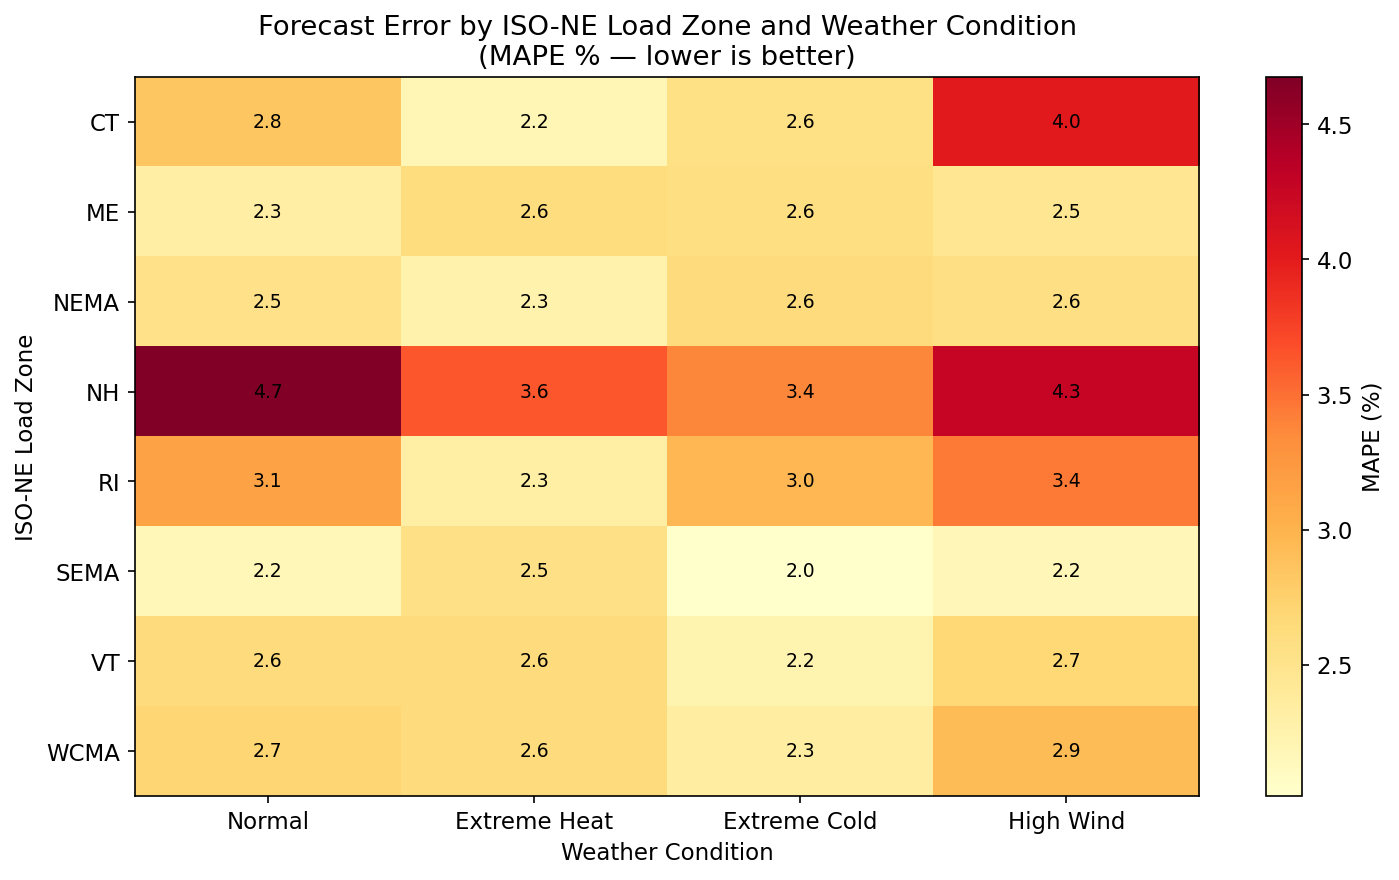
\includegraphics[width=0.92\linewidth]{part3/results/figures/fig3_stratified_mape_heatmap.png}
    \caption{MAPE by ISO-NE zone and weather bucket.}
    \label{fig:part3-heatmap}
\end{figure}

\begin{figure}[t]
    \centering
    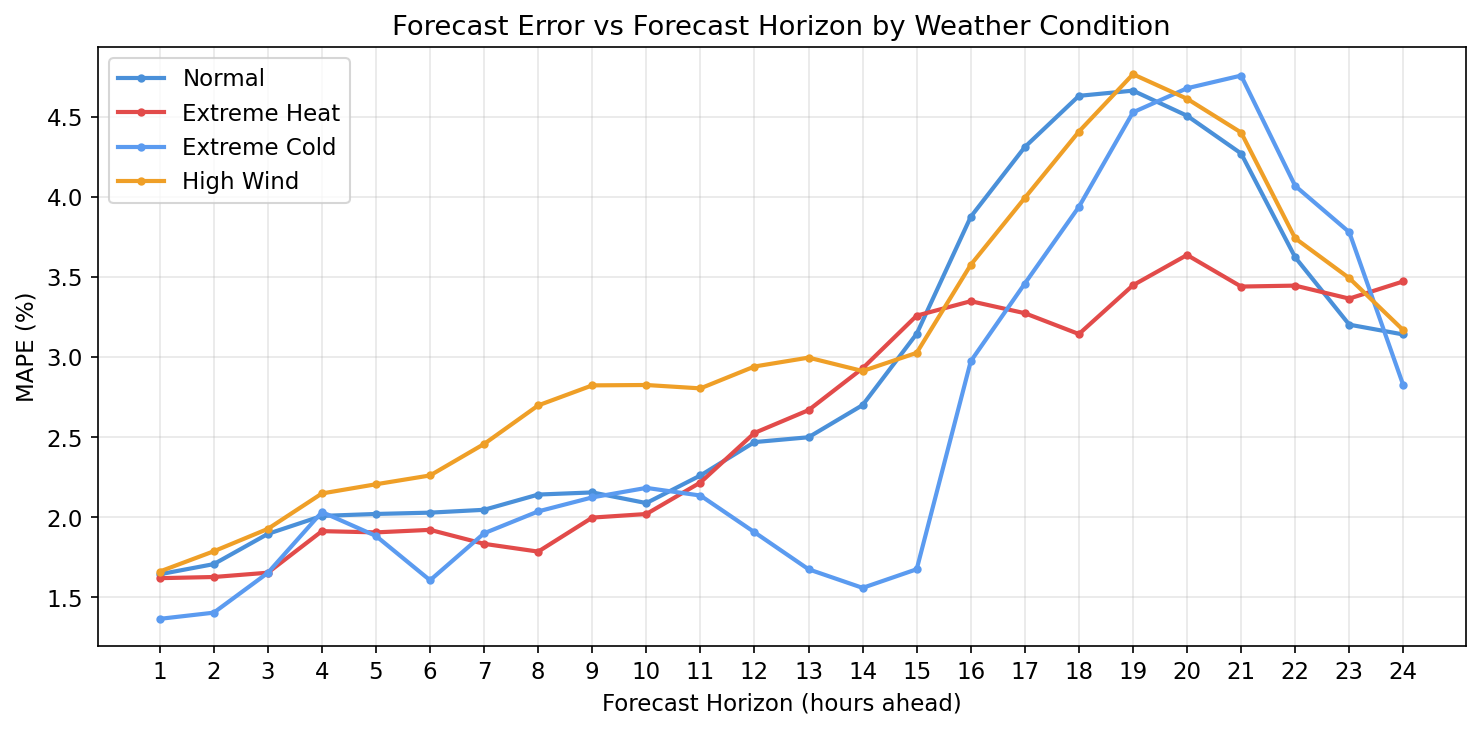
\includegraphics[width=0.92\linewidth]{part3/results/figures/fig4_horizon_curves.png}
    \caption{Forecast-horizon error curves by weather bucket.}
    \label{fig:part3-horizon}
\end{figure}

\begin{figure}[t]
    \centering
    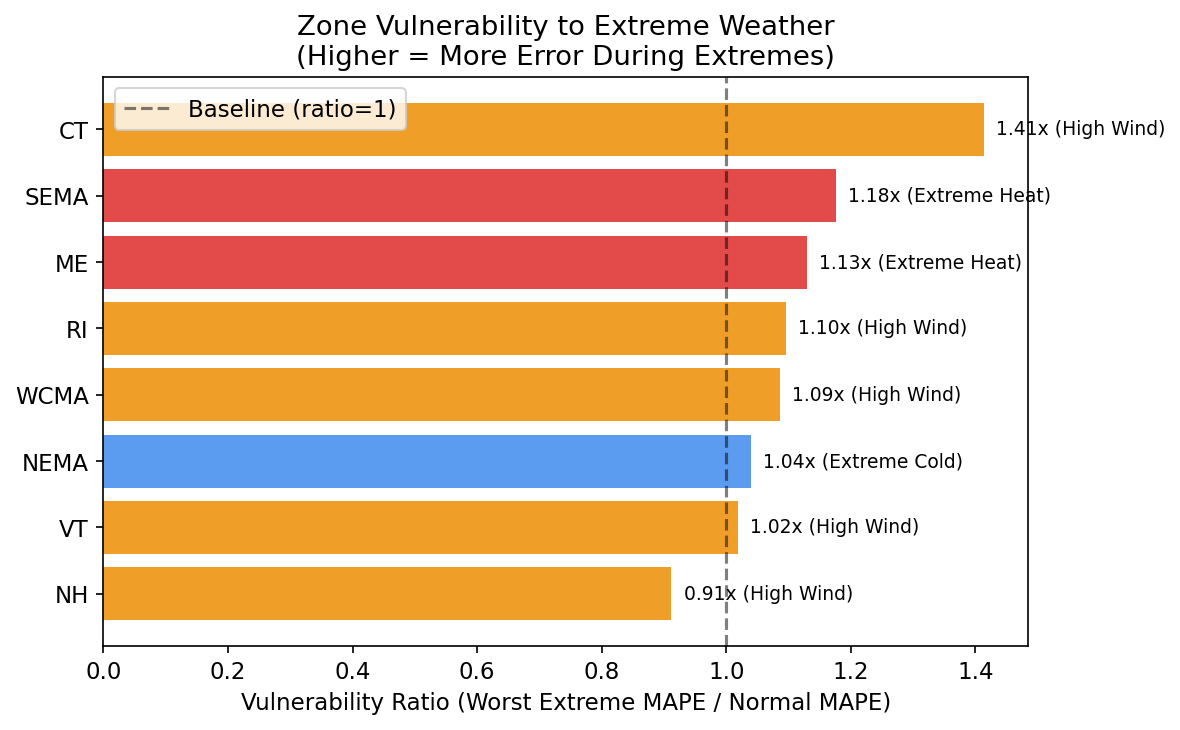
\includegraphics[width=0.78\linewidth]{part3/results/figures/fig5_zone_vulnerability_ranking.png}
    \caption{Zone vulnerability ranking based on the ratio of worst extreme-weather MAPE to normal MAPE.}
    \label{fig:part3-ranking}
\end{figure}

\subsection{Discussion and Policy Implications}
\label{subsec:part3-discussion}

The practical implication is that robustness is not evenly distributed. The model is not simply ``bad'' during extreme weather; rather, it fails in specific places and under specific conditions. That pattern suggests targeted operational responses. For cold-sensitive zones such as ME, NEMA, and SEMA, operators should prioritize winter preparedness, local demand-response readiness, and more granular weather inputs near the coast and in colder northern areas. For CT and the high-wind regime, additional wind-sensitive sensing and horizon-specific calibration may be useful. For ME and VT during heat events, the error increase suggests that the model may be missing local demand amplification that only appears in rare summer stress periods.

\subsection{Limitations}
\label{subsec:part3-limitations}

This analysis is limited by event rarity, especially for winter storms, which leaves some buckets underpowered. The proxy evaluation uses 2022--2023 rather than the hidden 2024 test set, so the final numerical values should be interpreted as a robustness study rather than the official benchmark result. Finally, the 450\times 449 weather grid may still smooth over micro-climate effects that matter at the zone level.
